\DiaryEntry{Inside Interesting Integrals, Flipside of Feyman's Trick (Section 3.4)}{2022-05-25}{Integrals}

This is a new trick and we'll use it to calculate the following integral,

\bee
I(a,b) = \int_0^\infty \frac{\cos(ax) - \cos(bx)}{x^2} dx
\eee

The trick is to express the integrand by means of an integral according to

\bee
\frac{\cos(ax) - \cos(bx)}{x^2} = - \int_b^a \frac{\sin(xy)}{x}dy
\eee

Keep in mind that we are integrating wrt to \emph{y}; the $x$ is therefore just a factor and we integrate $\sin(xy)$ wrt to $y$. Inserting this into the original expression, we obtain

\bee
I(a,b) = - \int_0^\infty \left( \int_b^a \frac{\sin(xy)}{x}dy \right) dx
\eee

This looks more complex, but we can exchange the order of integrals and (in this case) this allows integration. So we have

\bee
I(a,b) = - \int_b^a \left( \int_0^\infty \frac{\sin(xy)}{x}dx \right) dy
\eee

From \eqref{2022-04-05:eq2} we know that

\bee
\int_0^\infty \frac{\sin ax}{x} dx =
\begin{cases} \frac{\pi}{2}, \quad a > 0 \\
    0, \quad a = 0 \\
    -\frac{\pi}{2}, \quad a < 0
\end{cases}
\eee

and we therefore have

\bee
I(a,b) = - \int_b^a \frac{\pi}{2} dy = \frac{\pi}{2} (b-a)
\eee

So we have

\bee\boxed{
  I(a,b) = \int_0^\infty \frac{\cos(ax) - \cos(bx)}{x^2} dx = \frac{\pi}{2} (b-a)
  } \qed
\eee

In a similar spirit, we can use an existing integral, sneak in some parameter, integrate over the parameter, exchange integrals, and see what happens. Here we go.

We have

\bee
\int_0^\infty e^{-x^2} dx = \frac{1}{2} \sqrt{\pi}
\eee

Let's parametrize this via $x = t \sqrt{a}$, therefore $dx = \sqrt{a}$ and therefore

\bee
\int_0^\infty e^{-a t^2} \sqrt{a} dt = \frac{1}{2} \sqrt{\pi} \rightarrow \int_0^\infty e^{-a t^2} dt = \frac{1}{2} \sqrt{\frac{\pi}{a}}
\eee

Next we integrate both sides wrt $a$ from $p$ to $q$ and obtain

\bee
\int_p^q \left( \int_0^\infty e^{-a t^2} dt \right) da = \int_p^q \frac{1}{2} \sqrt{\frac{\pi}{a}} da = \cdots = \sqrt{\pi} (\sqrt{q} - \sqrt{p})
\eee

Now let's reverse the order of integration. We obtain

\bee
\int_0^\infty \left( \int_p^q e^{-a t^2} da \right) dt = \int_0^\infty \left( \frac{1}{t^2} \left. e^{-a t^2} \right|_p^q \right) dt = \int_0^\infty \frac{e^{-q t^2} - e^{-p t^2} }{t^2} dt
\eee

Combining this yields the following result,

\bee\boxed{
  \int_0^\infty \frac{e^{-q t^2} - e^{-p t^2} }{t^2} dt = \sqrt{\pi} (\sqrt{q} - \sqrt{p})
  }
\eee

The following Figure shows plots of the three functions $e^{-2x^2}/x^2$ (blue), $e^{-x^2}/x^2$ (red), and $(e^{-x^2} - e^{-2x^2})/x^2$ (green). The pole of $e^{-qx^2}/x^2$ at $x=0$ is compensated in the integrand and in the limit $x=0$ we have

\begin{align*}
  \lim_{t \rightarrow 0} \frac{e^{-q t^2} - e^{-p t^2} }{t^2} &= \lim_{t \rightarrow 0} \left( \frac{1}{x^2} - q + \frac{q^2x^2}{2} + \cdots \right) - \left( \frac{1}{x^2} - p + \frac{p^2x^2}{2} + \cdots \right)\\
  &= \lim_{t \rightarrow 0} \left( \frac{1}{x^2} - \frac{1}{x^2} -q + p + \frac{q^2x^2}{2} - \frac{p^2x^2}{2} + \cdots \right) = p-q
\end{align*}

In the exmaple we have $p=1, q=2$ and therefore the integrand becomes $p-q=1$ at $x=0$.

\begin{figure}[H]
    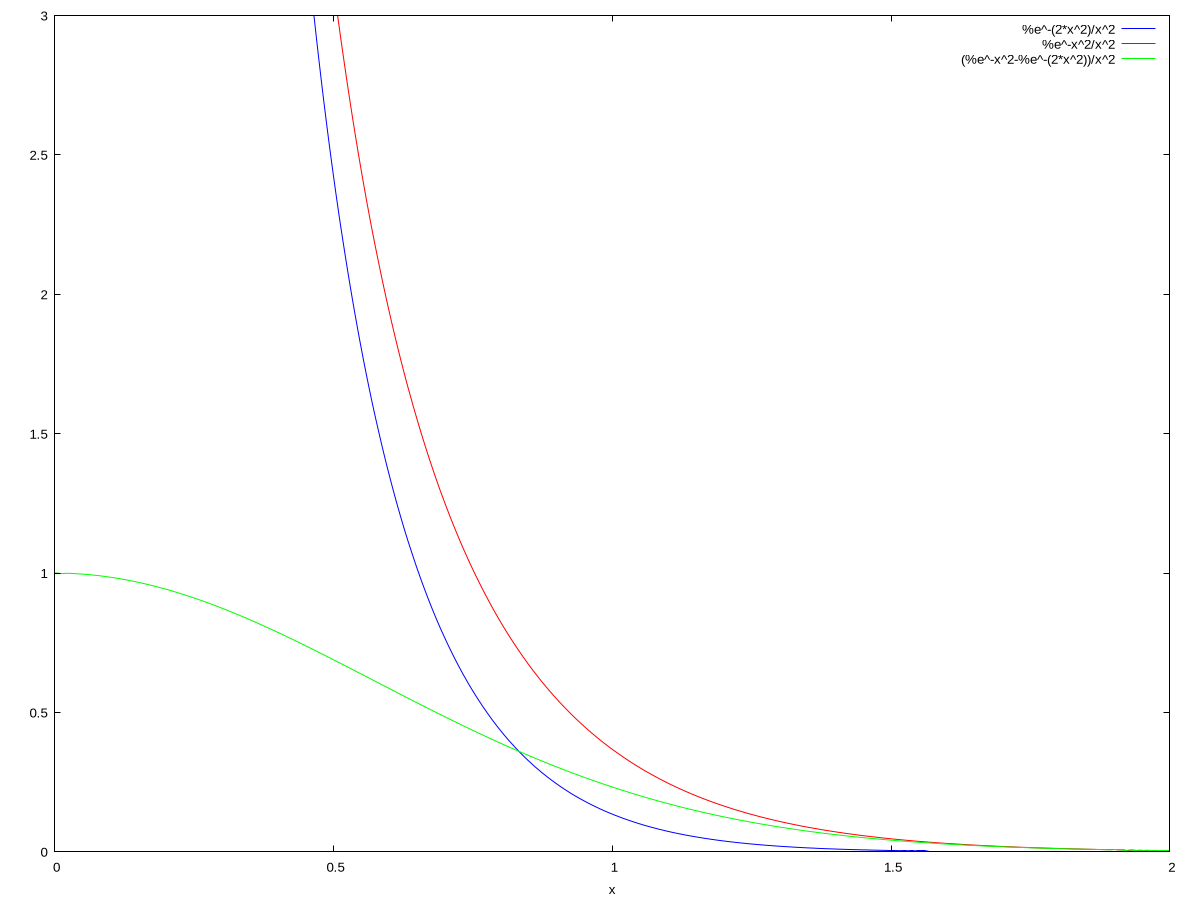
\includegraphics[scale=0.35]{images/2022-05-25-plot_1.png}
\end{figure}

  
%%% Local Variables:
%%% mode: latex
%%% TeX-master: "journal"
%%% End:
